

\documentclass[10pt]{extarticle}

\usepackage[utf8]{inputenc}
\usepackage{extsizes} % Allow for more sizes suchas 14pt or 17pt on document class.
\usepackage{mathtools} % Allows conditional math expressions, etc.

% Don't output references in case they're empty - http://tex.stackexchange.com/questions/74476/how-to-avoid-empty-thebibliography-environment-bibtex-if-there-are-no-refere

\let\myBib\thebibliography
\let\endmyBib\endthebibliography

\renewcommand\thebibliography[1]{\ifx\relax#1\relax\else\myBib{#1}\fi}


\begin{document} 



%% Front page.
\title{Advise for Applying Machine Learning}

    
    \date{}
    

    

    \maketitle

\newpage
%% Abstract page.


%% Table of contents page.



%% Body start.
\section{Deciding What to Try Next.}\label{deciding-what-to-try-next.}

Introduction: In this section how to not waste time choosing / debugging
algorithms will be explained.

Example: Say that we have a regularized linear regression
implementation, and it makes unacceptably large errors. What should we
do?

\begin{itemize}
\itemsep1pt\parskip0pt\parsep0pt
\item
  More training examples? Might not be the best idea - can waste time.
\item
  Try smaller sets of features. Might prevent overfitting.
\item
  Try getting additional features. We can waste time - need to know if
  it will work.
\item
  Try additional features.
\item
  Decreasing, increasing $\lambda$.
\item
  etc\ldots{}.
\end{itemize}

We can waste a lot of time doing this if we are not sure why our
algorithm fails, so we're gonna try to see what shall be the best
option, or at least rule out some of them so we don't lose time doing
something that is not going to increase the prediction accuracy.

The tests done to solve this problems will be called \textbf{Machine
learning diagnostic tests}.

\section{Evaluating a Hypothesis}\label{evaluating-a-hypothesis}

How do you tell if a hypothesis is overfitting?\\Just split the data in
two portions: The first portion is going to be the training set and the
other one the test set (70\%-30\% split is a good estimation).

We train with the training data and evaluate our model with the test
data. We can evaluate the model using different metrics, such as mse (eq
\ref{eq:mse}) for regression or the 1/0 error for classification (eq
\ref{eq:one_zero_error}).

\begin{equation} \label{eq:mse}
J_{test}(\theta) = \frac{1}{2m_{test}} \sum_{i=1}^{m_{test}}(h_\theta(x_{test}^{(i)}) - y_{test}^{(i)})^2
\end{equation}

\begin{equation} 
error(h_\theta(x), y) = 
\begin{dcases}
    1, & \text{if\,} h_\theta(x) \geq 0.5, y = 0 \\ 
       & \text{or\,} h_\theta(x) < 0.5, y = 1 \\
    0, & \text{otherwise}
\end{dcases} 
\end{equation}

\begin{equation} \label{eq:one_zero_error}
\text{test error} = \frac{1}{m_{test}} \sum_{i=1}^{m_{test}} error(h_\theta(x_{test}^{(i)}), y^{(i)})
\end{equation}

\section{Model Selection and Train/Validation/Test
Sets}\label{model-selection-and-trainvalidationtest-sets}

Say that we want to fit a problem. We want to decide the degree (d) of
the polynomial to use (amount of features extracted from a single
feature using the feature \^{}2, \^{}3, etc).

Each single polynomial will fit to different $\theta$ (d = 1 to
$\theta^{(1)}$, d = 2 to $\theta^{(2)}$, etc).

To find the best d, we could minimize the test error. If we do that,
though, what happens is that we would overfit the d parameter for the
test set, and we don't want to do that.

\subsection{Welcome, Cross Validation
set.}\label{welcome-cross-validation-set.}

In order to fix that problem, we simply split the data in 3: Training,
CrossValidation and Test (with a typical ratio of 60\% - 20\% - 20\%).
The CV error is calculated with the same formulas, only with the CV
data, obviously.

Once we have that split, we train every different model (each with a
different d) and choose the one that has the lowest CV error. This way,
we can still use the test error in order to know whether our model is
overfitting on ``real life'' data.

\section{Diagnosting Bias
vs.~Variance}\label{diagnosting-bias-vs.variance}

We continue with the example of the previous section.

When we increase the degree of the polynomial, we get less error on the
training set, which means we're overfitting. With the CV/Test sets,
though, the error increases at a certain point, where the model fails to
generalize the data (overfitting).

When we have a high CV error, we can have either high variance or high
bias. High bias - Underfitting is when both training error and CV error
are high. On the other hand, High variance - Overfitting is when
training error is very low and the CV error is high.

We can see all these in figure \ref{fig:error_degree_polynomial}.

\begin{figure}
\centering
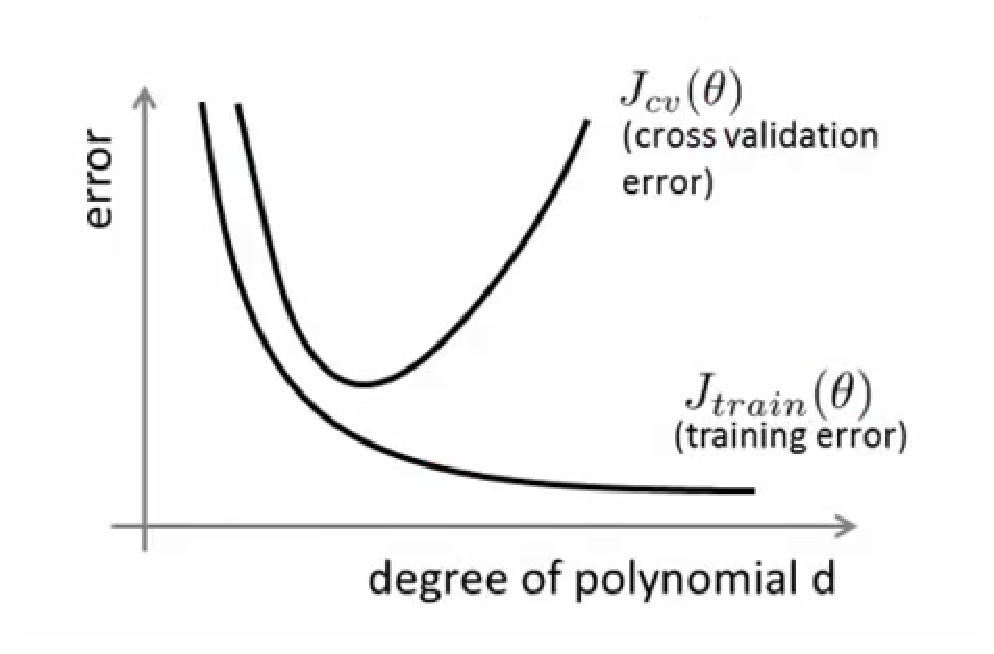
\includegraphics[width=\textwidth]{img/error_degree_polynomial.eps}
\caption{Error on degree of the polynomial.}
\label{fig:error_degree_polynomial}
\end{figure}

\section{Regularization and
Bias/Variance}\label{regularization-and-biasvariance}

Suppose we're fitting a high order polynomial with regularization to
evade the overfitting trap.

In figure \ref{fig:lambda_bias_variance} we can see that, given the case
of a high order polynomial, when we have a large $\lambda$ we are
underfitting the data and when we have a small $\lambda$ we're
overfitting it.

\begin{figure}
\centering
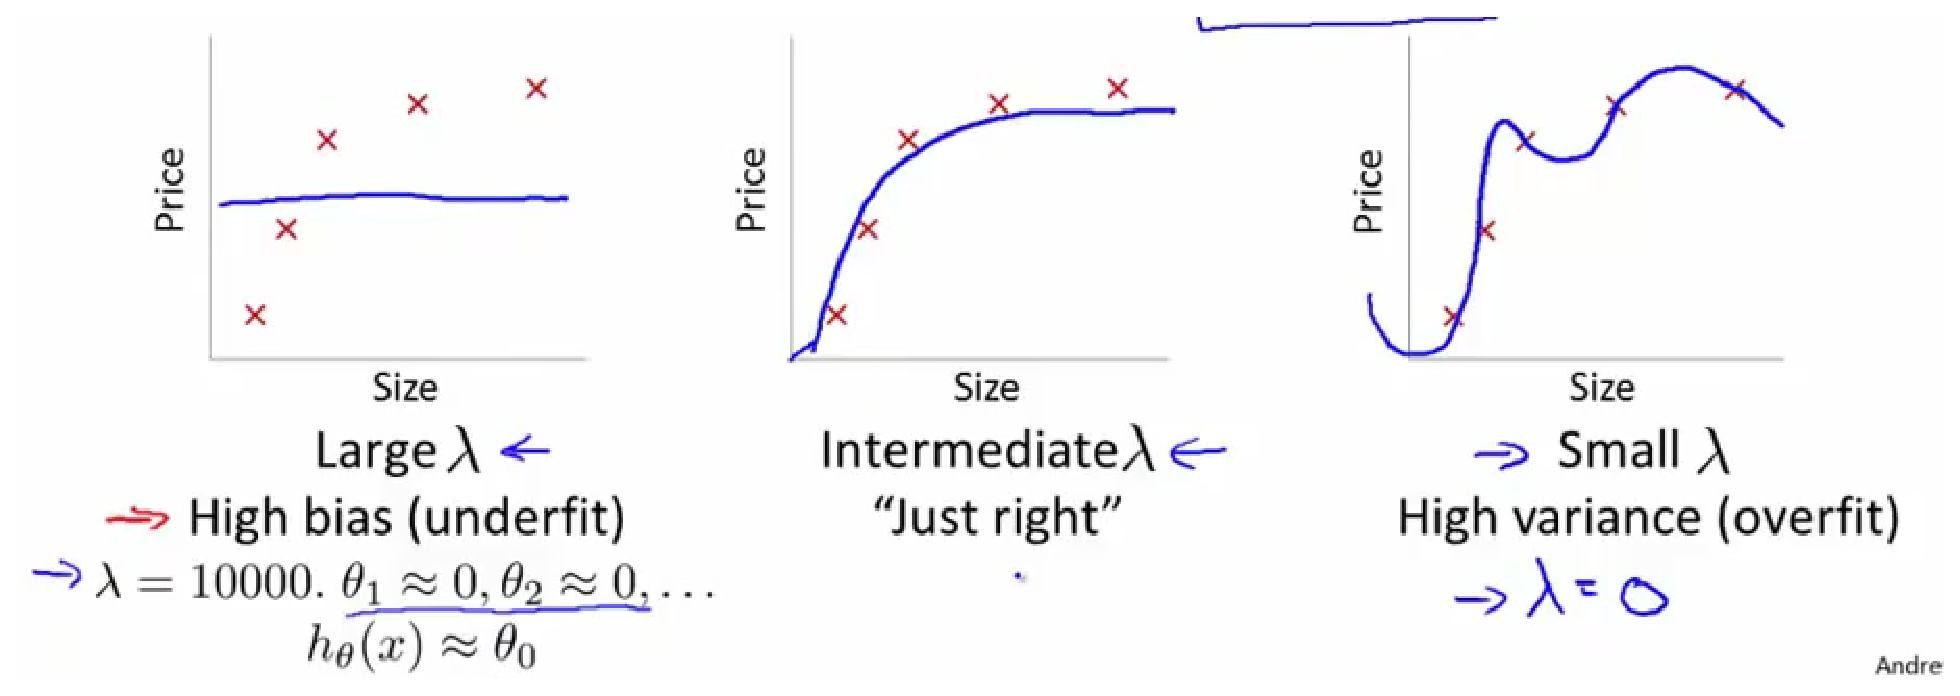
\includegraphics[width=\textwidth]{img/lambda_bias_variance.eps}
\caption{Different $\lambda$ values comparisson on a high degree polynomial.}
\label{fig:lambda_bias_variance}
\end{figure}

An important detail here is noticing that, even though we use
regularization when training, we don't use it for the evaluation cost
functions, where we use the simple mse function (equation \ref{eq:mse}).

In order to find the correct $\lambda$ value, we train a model with
every different value and pick up the one that gives the min CV error
function. We can then evaluate the chosen $\theta$ with the test error
function to see how well it's working (figure
\ref{fig:lambda_cv_train_error}).

\begin{figure}
\centering
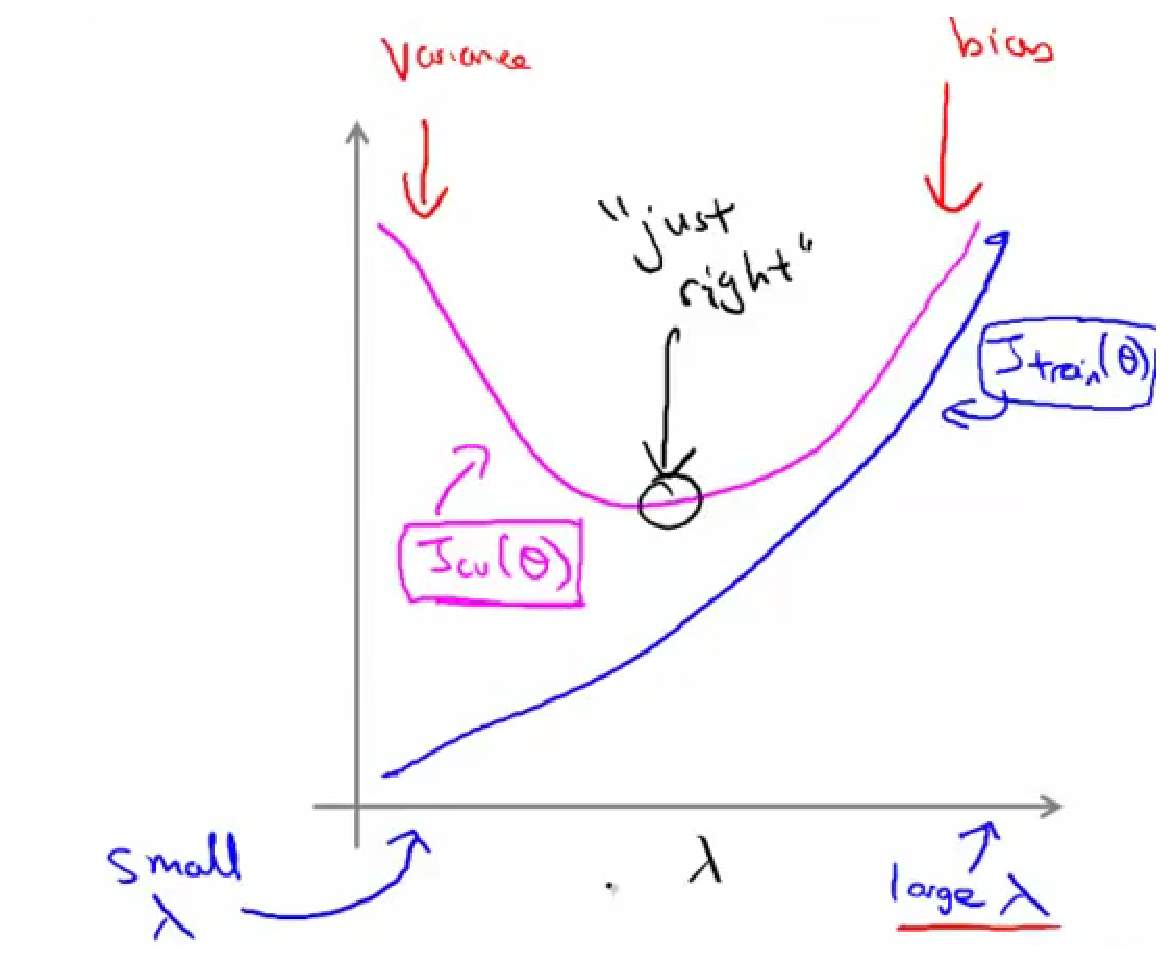
\includegraphics[width=\textwidth]{img/lambda_cv_train_error.eps}
\caption{CV and Train error functions related to $\lambda$ values.}
\label{fig:lambda_cv_train_error}
\end{figure}

\section{Learning Curves}\label{learning-curves}

Tool to diagnose a algorithm and find out if it suffers from bias or
variance.

Artificially reduce training set size and train with that. On very small
datasets the training error will be very small because it will fit
perfectly. As the size of the dataset increases, though, the training
error increases.

With the CV error, it starts with huge errors when training with a small
dataset and then the error decreases as the training set size increases.

We can see the ``perfect'' graph we should expect if our model isn't
overfitting or underfitting the data in figure
\ref{fig:error_training_size_perfect}.

\begin{figure}
\centering
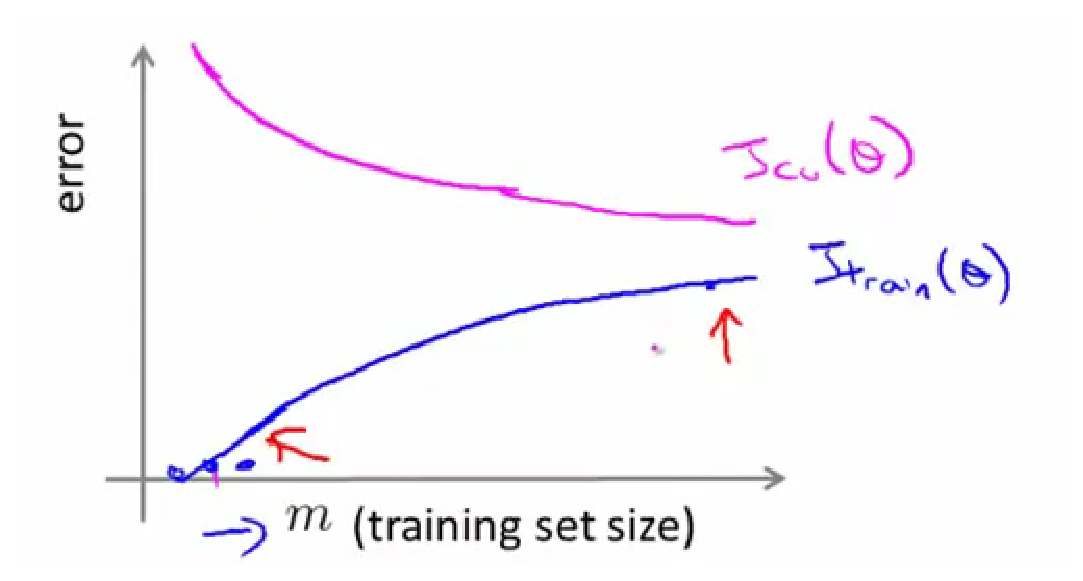
\includegraphics[width=\textwidth]{img/error_training_size_perfect.eps}
\caption{Error on training set size without both variance and bias.}
\label{fig:error_training_size_perfect}
\end{figure}

If we have high bias (underfitting), the cross validation error will end
up close to the train error (figure \ref{fig:error_training_size_bias}).
This means that if we have a high bias, getting more data doesn't help
much.

\begin{figure}
\centering
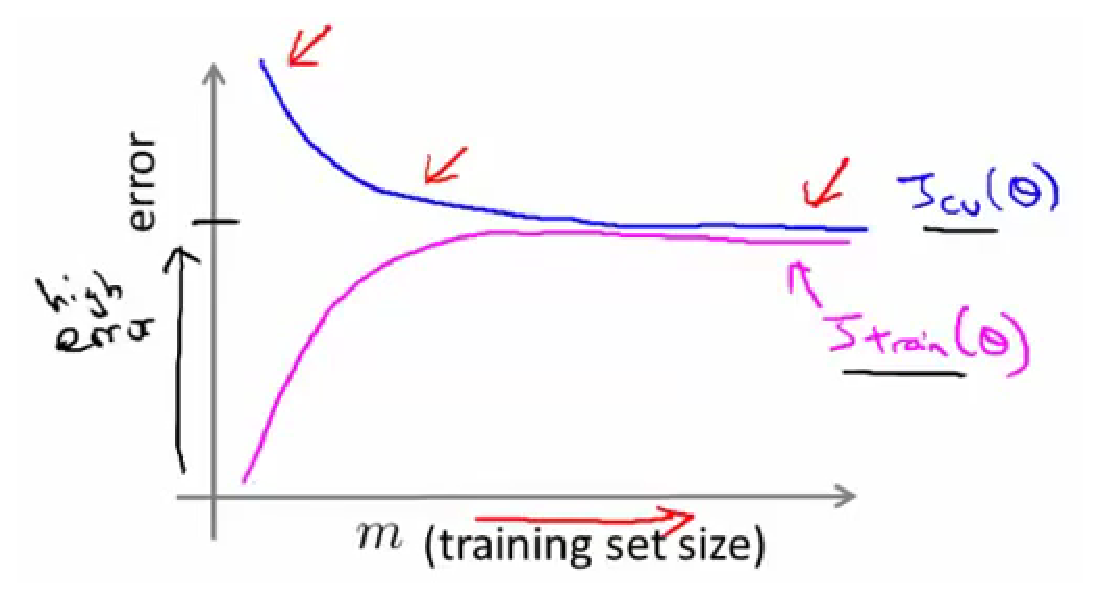
\includegraphics[width=\textwidth]{img/error_training_size_bias.eps}
\caption{Error on training set size with bias (underfitting).}
\label{fig:error_training_size_bias}
\end{figure}

If we have high variance (overfitting), the model will have a very low
training error and very high CV error (figure
\ref{fig:error_training_size_variance}). In this case, getting more data
is likely to help.

\begin{figure}
\centering
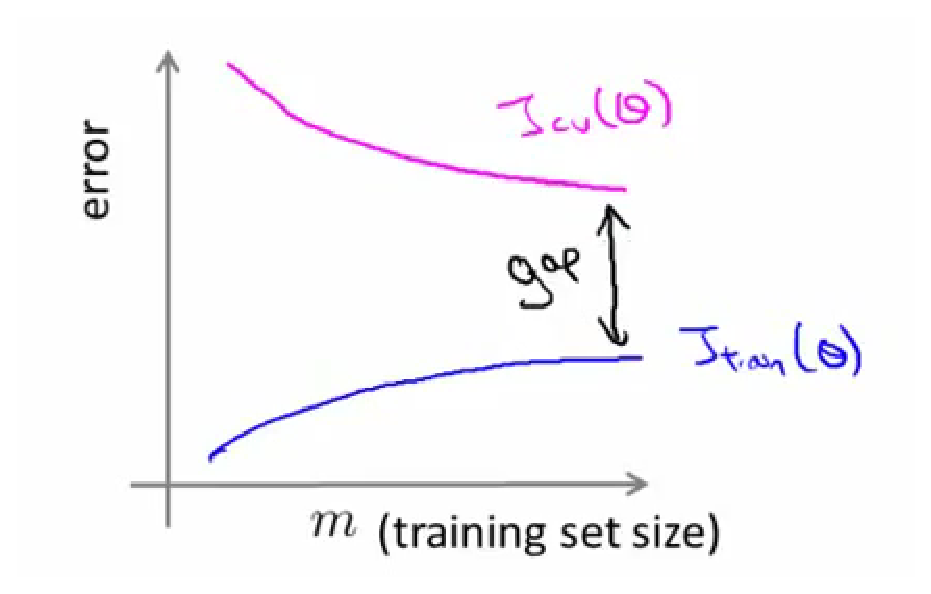
\includegraphics[width=\textwidth]{img/error_training_size_variance.eps}
\caption{Error on training set size with variance (overfitting).}
\label{fig:error_training_size_variance}
\end{figure}

\section{Deciding What to Do Next
Revisited}\label{deciding-what-to-do-next-revisited}

\begin{itemize}
\itemsep1pt\parskip0pt\parsep0pt
\item
  Getting more training examples $\rightarrow$ Fixes high variance.
\item
  Smaller sets of features $\rightarrow$ Fixes high variance.
\item
  Additional features $\rightarrow$ Fixes high bias.
\item
  Adding polynomial features $\rightarrow$ Fixes high bias.
\item
  Decreasing $\lambda$ $\rightarrow$ Fixes high bias.
\item
  Increasing $\lambda$ $\rightarrow$ Fixes high variance.
\end{itemize}

\subsection{Neural Networks}\label{neural-networks}

A small neural network is prone to underfitting and a large one is prone
to overfitting.


%% Body end.

%% Bibliography.

    \nocite{*}

\bibliographystyle{plain}
\bibliography{references}

\end{document}